\chapter{Testing and User Feedback}
\label{cha:testing}

Testing is an important facet of any programming. It ensures that the code is functional and free from logical errors.
Test-driven development (TDD) is the practice of writing unit tests before implementing a feature or bug fix, allowing developers to define exactly how a specific function is expected to work given a set of inputs before focusing on how the function achieves the correct outputs.
Defect rates have been shown to decrease by around 50\% when following TDD, compared to a traditional style of testing, where tests are written after the fact \citep{maximilien2003assessing}.

\section{Unit Testing}
Unit tests are a fundamental form of testing for all applications. They are small, focused tests that verify the correctness of individual components of a system.
Each test checks whether a specific function produces the expected outputs, given a set of inputs.
Unit tests are reusable by design, building into a suite of tests that are quick to run over time and ensure regressions do not occur.
Regression tests are particularly valuable as they increase confidence that new changes do not break existing features unexpectedly.
The field of regression testing and minimisation of regression tests is vast.
However, much work has been done to automate the selection of regression tests to keep overall costs (time and energy) down whilst still providing a comprehensive suite of tests which aim to cover as much of the application as possible \citep{wong1997study}. 

Omni utilises unit tests to cover most of the codebase, aiming for code coverage of over 70\% but achieving close to 100\% across the key, testable areas of the codebase (shown in Figure \ref{fig:test-coverage}).

\begin{figure}[htbp]
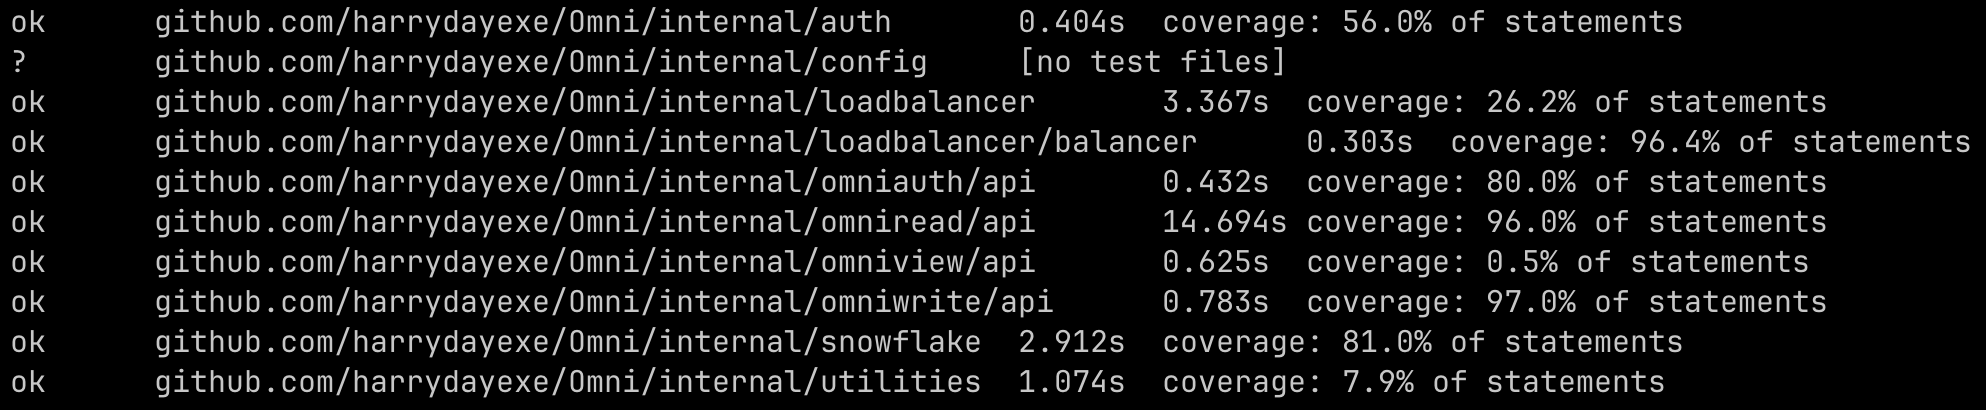
\includegraphics[width=12cm]{test-coverage.png}
\centering
\caption{Omni Test Coverage Report}
\label{fig:test-coverage}
\end{figure}

Demanding code coverage requirements (such as enforcing all code to be at least 70\% covered) is less effective and even detrimental to the actual defect rates of codebases.
Instead, it is more effective to encourage practitioners to focus on more in-depth code coverage metrics such as Modified Condition-Decision (MC/DC) coverage, which is much more effective at highlighting faults before they become user-facing errors \citep{hemmati2015effective}. 

\section{Integration Testing}
The second important aspect of testing is the use of integration tests. Unit tests, whilst powerful and robust, are inherently limited in scope.
To keep them self-contained and fast to execute, they should not interact with external services such as databases or APIs. This limitation is where integration tests shine.

As the name implies, the design of an integration test allows them to test how different sections (or units) of the system integrate.
Integration can include how an application interacts with a real database or external API.
Integration tests do not have the same expectations about runtime and, in some cases, can take minutes or even hours to execute more complex scenarios.
However, they should still enforce the same requirements around repeatability and reusability, again to build up a suite of test cases for a product to pass before an update ships to market. 

Whereas unit tests should be run consistently by the engineer throughout the development lifecycle, integration tests are usually only run after an engineer is confident in their work, often by a CI/CD tool.

\subsection{Testcontainers}
Engineers often face the challenge of ensuring that the integration tests they write are repeatable.
For example, a database needs to be reset to a common starting point before each run of the tests to ensure consistency across iterations. 

In 2015, an open-source project called \underline{\href{https://testcontainers.com}{Testcontainers}} \nocite{testcontainers} was released to the public, intending to solve just that issue.
Taking the example of an integration test that interacts with a database, instead of running the tests against a permanent database, which would need to be reset and modified after each run, the Testcontainers framework allows the creation of a database inside a container.
Each integration test can be run in parallel, connecting to different containers, ensuring that side effects from one test do not affect another. 

Because each test can define its dependencies in a container(s), the setup for each dependency is explicitly set in code and portable for any developer to run.
This allows integration tests to be run locally on an engineer's computer or in a larger CI/CD pipeline. 

Adopting Testcontainers for integration tests requires just a few lines of code to configure the container in each test case.
It brings all the benefits that ensure tests are repeatable, consistent and not flaky.

OmniRead utilises Testcontainers for integration testing between the request handlers and the underlying database logic, verifying that the queries written are accurate and valid.
A unit test cannot check the SQL queries themselves as the database layer is mocked to ensure speed when running the test suite.
Figure \ref{fig:testcontainers}\footnote{The ryuk container runs for the duration of the test suite and is responsible for killing any containers that are not terminated by the test suite itself (for example if one of the tests fails early)} shows the containers created as part of the integration test suite, demonstrating the parallelisation possible due to each test running on a fundamentally different database.

\begin{figure}[htbp]
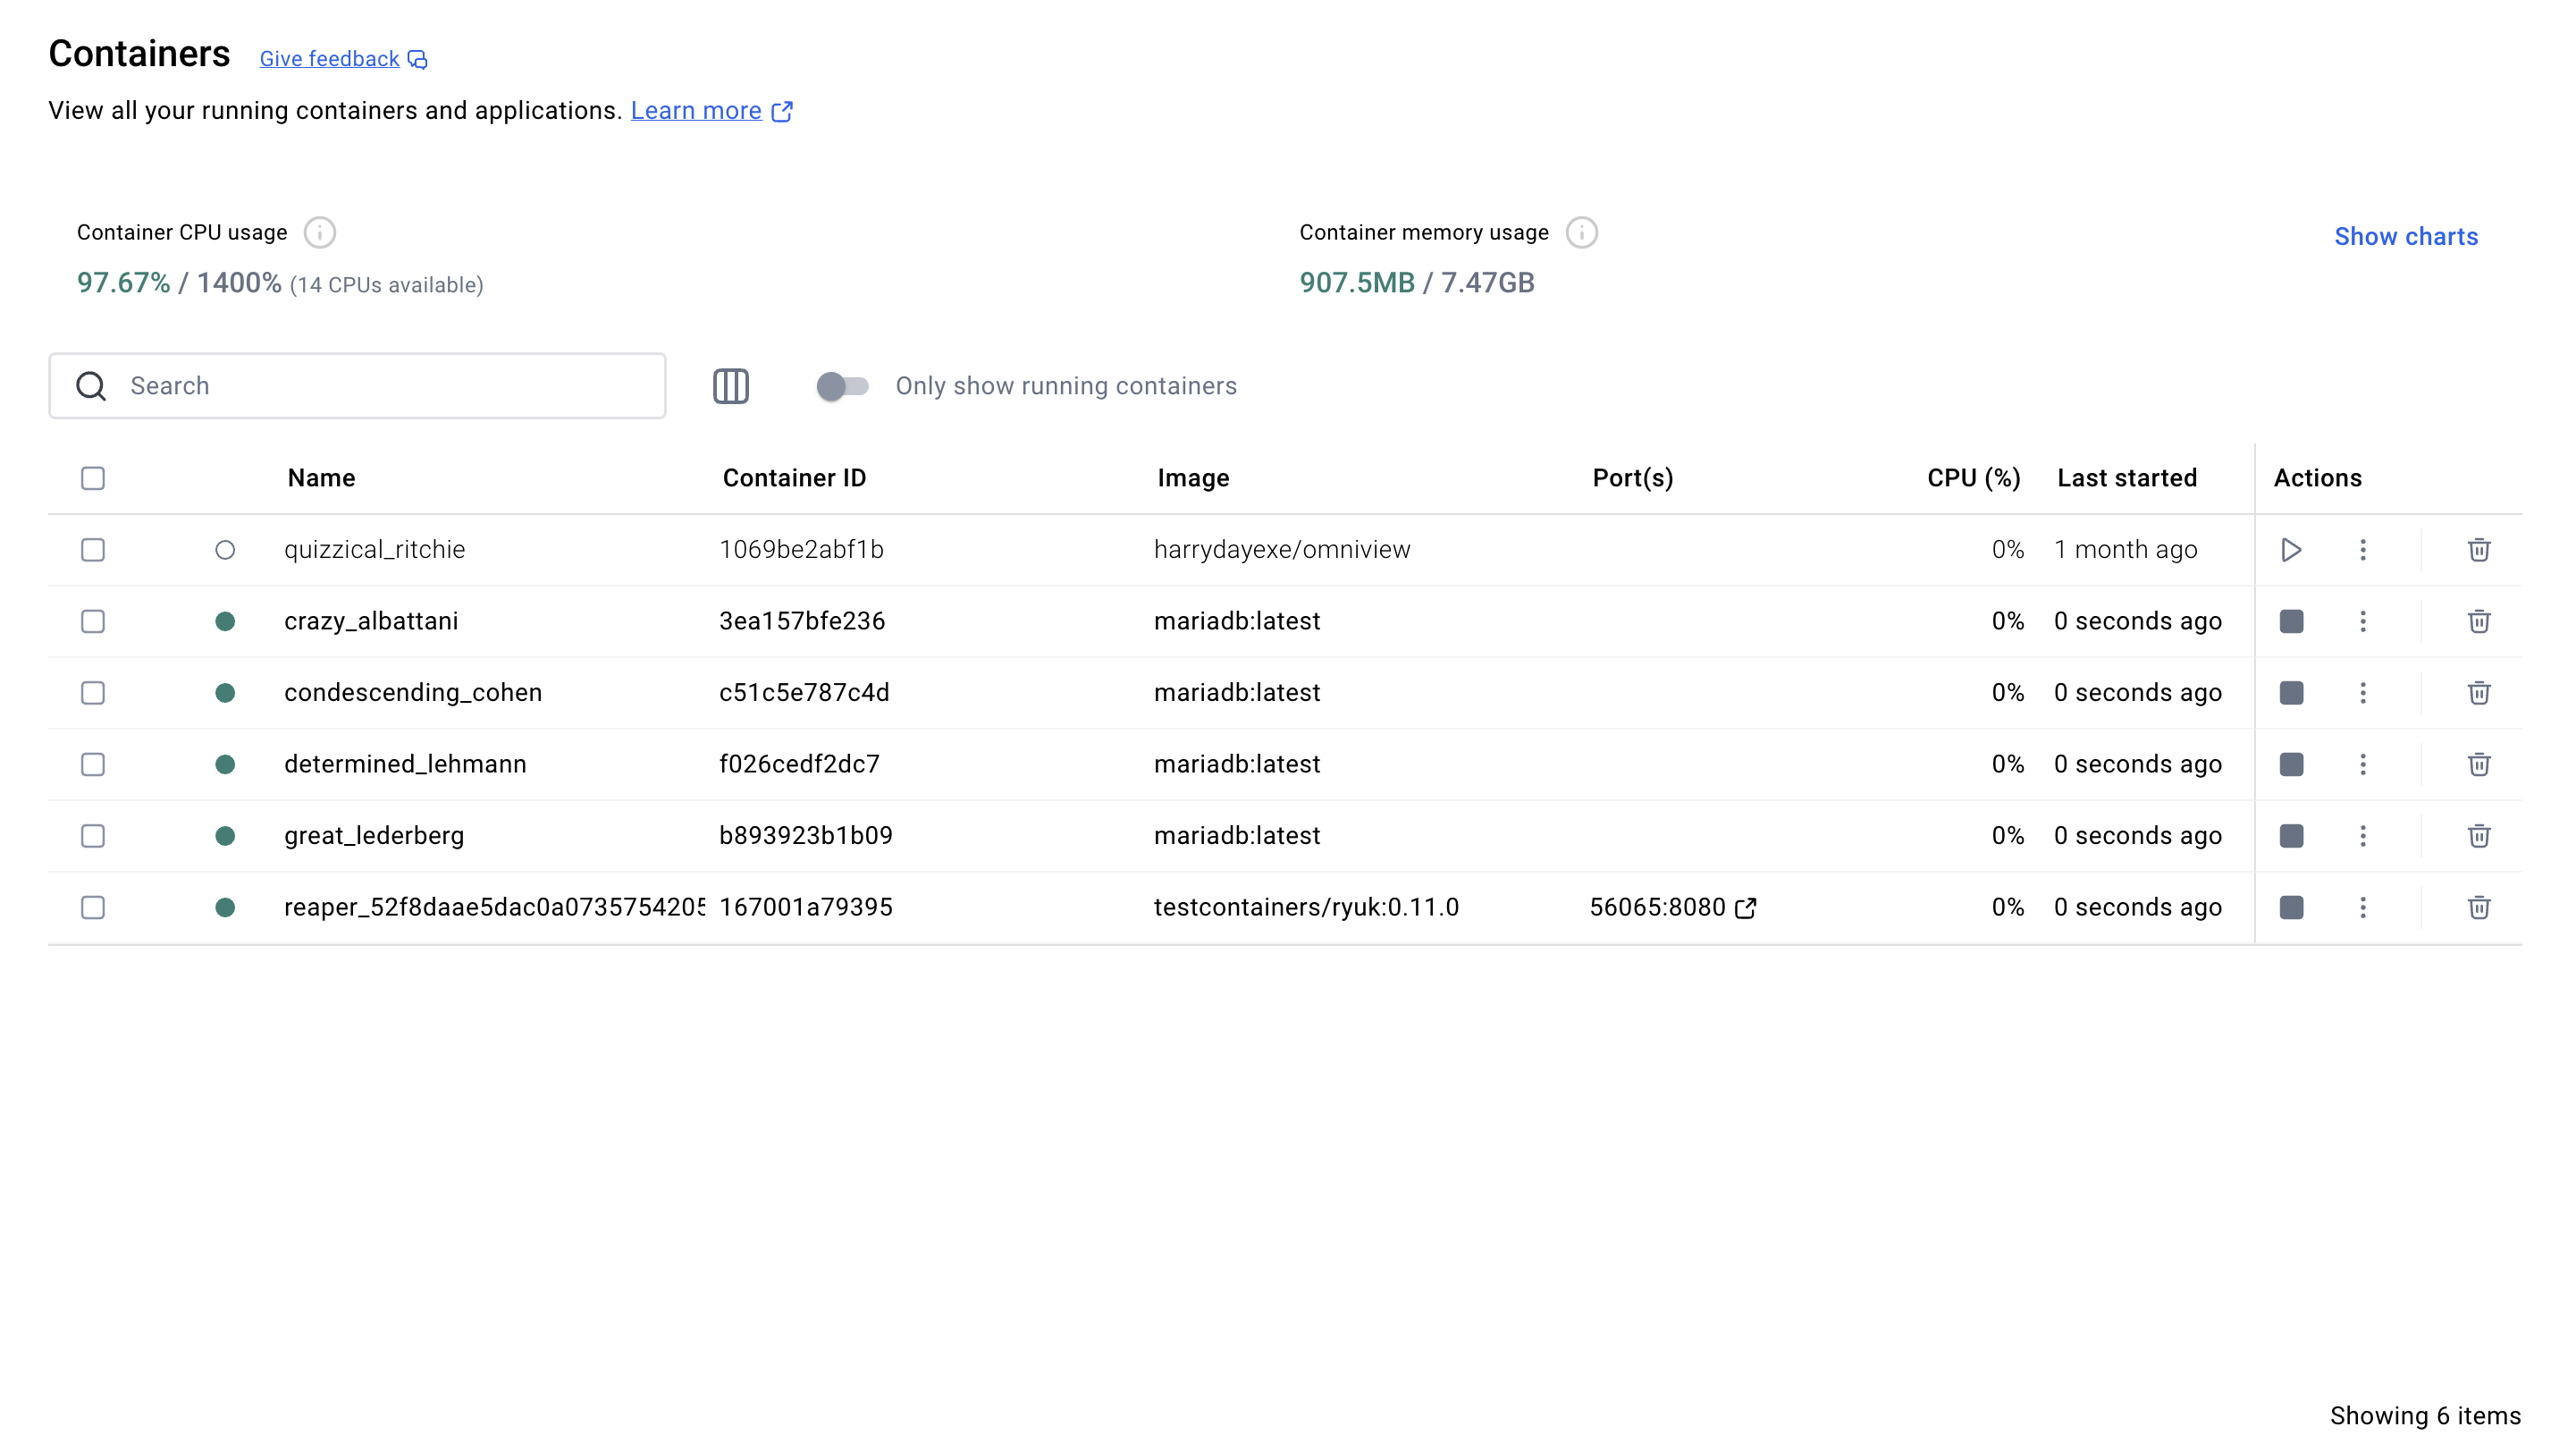
\includegraphics[width=12cm]{testcontainers.png}
\centering
\caption{Testcontainers Running during the Integration Tests}
\label{fig:testcontainers}
\end{figure}
